\documentclass[11pt, leqno]{scrartcl}
\usepackage{polski}
\usepackage[polish]{babel}

\usepackage{graphicx, float, caption, subcaption, amsmath}
\usepackage{tabularx, multirow, hyperref, enumitem, listings}
\usepackage{xcolor}
%\usepackage{minted}

\hypersetup{
    colorlinks=true,
    linkcolor=black,
    urlcolor=black,
    citecolor=black
}

\definecolor{md-black}{rgb}{0.12, 0.12, 0.12}
\definecolor{md-teal}{rgb}{0.38, 0.79, 0.69}
\definecolor{md-mauve}{rgb}{0.76, 0.52, 0.75}
\definecolor{md-yellow}{rgb}{0.86, 0.86, 0.67}
\definecolor{md-green}{rgb}{0.13, 0.55, 0.13}
\definecolor{md-red}{rgb}{0.82, 0.10, 0.14}
\definecolor{md-purple}{rgb}{0.69, 0.33, 0.73}
\definecolor{md-orange}{rgb}{0.96, 0.42, 0.18}
\definecolor{md-gray}{rgb}{0.44, 0.46, 0.51}
\lstset{
    language=Python,
    basicstyle=\color{md-teal}\ttfamily,
    keywordstyle=\color{md-mauve},
    commentstyle=\color{md-green},
    stringstyle=\color{md-red},
    numbers=left,
    numberstyle=\small\color{md-gray}\ttfamily,
    stepnumber=1,
    numbersep=5pt,
    backgroundcolor=\color{md-black},
    showspaces=false,
    showstringspaces=false,
    showtabs=false,
    frame=none,
    tabsize=4,
    captionpos=b,
    breaklines=true,
    breakatwhitespace=false,
    escapeinside={\%*}{*)},
    numbersep=-10pt,
    morekeywords={as},
    classoffset=1,
    morekeywords={quad, quad_vec, trapz, simps, linregress,
        newton},
    keywordstyle=\color{md-yellow},
    classoffset=0
}

\graphicspath{{../images/}}

\title{Laboratorium 8 - Rozwiązywanie równań nieliniowych}
\author{Mateusz Podmokły - II rok Informatyka WI}
\date{25 kwiecień 2024}

\begin{document}
    \maketitle
    \section{Treść zadania}
    \textbf{Zadanie 1.}
    Dla poniższych funkcji i punktów początkowych metoda
    Newtona zawodzi. Wyjaśnij dlaczego. Następnie znajdź
    pierwiastki, modyfikując wywołanie funkcji
    \texttt{scipy.optimize.newton} lub używając innej
    metody.
    \begin{align*}
        &f_1(x)=x^3-5x,x_0=1 \\
        &f_2(x)=x^3-3x+1,x_0=1 \\
        &f_3(x)=2-x^5,x_0=0.01 \\
        &f_4(x)=x^4-4.29x^2-5.29,x_0=0.8
    \end{align*}

    \subsection*{}
    \textbf{Zadanie 2.} Dane jest równanie:
    \[
        f(x)=x^2-3x+2=0
    \]
    Każda z następujących funkcji definiuje równoważny
    schemat iteracyjny:
    \begin{align*}
        &g_1(x)=\frac{x^2+2}{3}, \\
        &g_2(x)=\sqrt{3x-2}, \\
        &g_3(x)=3-\frac{2}{x}, \\
        &g_4(x)=\frac{x^2-2}{2x-3}
    \end{align*}
    Przeanalizuj zbieżność oraz rząd zbieżności schematów
    iteracyjnych odpowiadających funkcjom $g_i(x)$ dla
    pierwiastka $x=2$ badając wartość $|g'_i(2)|$. \\
    Potwierdź analizę teoretyczną implementując powyższe
    schematy iteracyjne weryfikując ich zbieżność (lub brak).
    Każdy schemat iteracyjny wykonaj przez 10 iteracji.
    Wyznacz eksprymentalnie rząd zbieżności każdej metody
    iteracyjnej ze wzoru
    \[
        r=\frac{ln\frac{\epsilon_k}{\epsilon_{k+1}}}
            {ln\frac{\epsilon_{k-1}}{\epsilon_k}}
    \]
    gdzie błąd bezwzględny $\epsilon_k$ definiujemy jako
    $\epsilon_k=|x_k-x_*|$, $x_k$ jest przybliżeniem
    pierwiastka w k-tej iteracji, a $x_*$ dokładnym
    położeniem pierwiastka równania. \\
    Na wspólnym rysynku przedstaw wykresy błędu względnego
    każdej metody w zależności od numeru iteracji. Użyj
    skali logarytmicznej na osi y (pomocna będzie funkcja
    \texttt{semilogy}). Stwórz drugi rysunek, przedstawiający
    wykresy błędu względnego tylko dla metod zbieżnych.

    \subsection*{}
    \textbf{Zadanie 3.} Napisz schemat iteracji wg metody
    Newtona dla każdego z następujących równań nieliniowych:
    \begin{align*}
        &f_1(x)=x^3-2x-5=0 \\
        &f_2(x)=e^{-x}-x=0 \\
        &f_3(x)=xsin(x)-1=0
    \end{align*}
    Jeśli $x_0$ jest przybliżeniem pierwiastka z dokładnością
    4 bitów, ile iteracji należy wykonać aby osiągnąć:
    \begin{itemize}
        \item 24-bitową dokładność
        \item 53-bitową dokładność?
    \end{itemize}

    \subsection*{}
    \textbf{Zadanie 4.} Napisz schemat iteracji wg metody
    Newtona dla następującego układu równań nieliniowych:
    \[
        x_1^2+x_2^2=1
    \]
    \[
        x_1^2-x_2=0
    \]
    Korzystając z faktu, że dokładne rozwiązanie powyższego
    układu równań to:
    \begin{align*}
        &x_1=\pm \sqrt{\frac{\sqrt{5}}{2}-\frac{1}{2}} \\
        &x_2=\frac{\sqrt{5}}{2}-\frac{1}{2}
    \end{align*}
    oblicz błąd względny rozwiązania znalezionego metodą
    Newtona.

    \section{Specyfikacja użytego środowiska}
    Specyfikacja:
    \begin{itemize}
        \item Środowisko: Visual Studio Code,
        \item Język programowania: Python,
        \item System operacyjny: Microsoft Windows 11,
        \item Architektura systemu: x64.
    \end{itemize}

    \section{Rozwiązanie problemu}
    \subsection{Biblioteki}
    W realizacji rozwiązania wykorzystane zostały następujące
    biblioteki:
    \begin{lstlisting}
        import numpy as np
        import matplotlib.pyplot as plt
        from scipy.optimize import newton
    \end{lstlisting}

    \subsection{Zadanie 1.}
    W celu poprawy działania metody Newtona dla funkcji
    $f_1,f_2,f_3,f_4$ zmodyfikowałem początkowe oszacowania
    $x_0$. Wykorzystana została do tego funkcja z biblioteki
    \texttt{SciPy}
    \[
        \texttt{scipy.optimize.newton}
    \]
    Przyjąłem następujące wartości $x_0$:
    \begin{align*}
        &f_1: \quad x_0\in \{-2,0,2\} \\
        &f_2: \quad x_0\in \{-2,0,2\} \\
        &f_3: \quad x_0=1 \\
        &f_4: \quad x_0\in \{-2,2\}
    \end{align*}
    Zaproponowane w zadaniu oszacowania $x_0$ nie były
    odpowiednie prawdopodobnie dlatego, że znajdowały się
    zbyt blisko ekstremum lokalnego funkcji.

    \subsection{Zadanie 2.}
    Badanie zbieżności za pomocą wzoru teoretycznego:
    \begin{align*}
        &|g'_1(2)|=1.33>1 &\text{(rozbieżny)} \\
        &|g'_2(2)|=0.75<1 &\text{(zbieżność liniowa)} \\
        &|g'_3(2)|=0.5<1 &\text{(zbieżność liniowa)} \\
        &|g'_4(2)|=0 &\text{(zbieżność wyższa niż liniowa)}
    \end{align*}
    Następnie zaimplementowałem te schematy iteracyjne
    i obliczyłem zbieżność ze wzoru
    \[
        r=\frac{ln\frac{\epsilon_k}{\epsilon_{k+1}}}
            {ln\frac{\epsilon_{k-1}}{\epsilon_k}}
    \]
    Wartość $r$ dla funkcji $g_1$ jest nieprzewidywalna
    i przyjmuje dodatnie oraz ujemne wartości, więc
    potwierdzony został brak zbieżności. \\
    Schemat iteracyjny funkcji $\sqrt{3x-2}$ nie jest
    zbieżny, ponieważ każda styczna do jej wykresu
    przecina oś OX poza dziedziną funkcji. W tej sytuacji
    zbieżność nie jest możliwa do wyznacznia za pomocą podanego
    wzoru. \\
    W przypadku funkcji $g_3$ punkty przecięcia
    stycznych z osią OX po każdej iteracji oddalają
    się od środka układu współrzędnych i od pierwiastka,
    więc schemat iteracyjny tej funkcji nie jest
    zbieżny. Tak samo jak wcześiej, nie jesteśmy w stanie wyznaczyć
    wartości zbieżności schematu iteracyjnego $r$. \\
    Dla ostatniej funkcji, w przypadku użycia metody
    Newtona, wartość $r$ zbiega do 0, co jest
    potwierdzeniem wcześniejszych obliczeń teoretycznych.
    
    \subsection{Zadanie 3.}
    Metoda Newtona została zaimplementowana zgodnie ze
    wzorem:
    \[
        x_{k+1}=x_k-\frac{f(x)}{f'(x)}
    \]
    gdzie $k$ to numer iteracji. \\
    Przeliczyłem dokładność w bitach na dokładność w cyfrach
    dziesiętnych - 24-bitową na 6 cyfr dziesiętnych,
    a 53-bitową na 14 cyfr. Iteracje metody Newtona były
    powtarzane do momentu uzyskania wymaganej dokładności.
    Liczba cyfr została obliczona według wzoru:
    \[
        d=-log_{10}\left| \frac{x_k-x_*}{x_*} \right|
    \]

    \subsection{Zadanie 4.}
    Możemy przekształcić równoważnie początkowy układ równań
    \[
        \begin{cases}
            x_1^2+x_2^2 = 1 \\
            x_1^2-x_2 = 0 \Rightarrow x_2=x_1^2
        \end{cases}
    \]
    \[
        \begin{cases}
            x_1^4+x_1^2-1=0 \\
            x_2=x_1^2
        \end{cases}
    \]
    Następnie do wzoru na metodę Newtona
    \[
        x_{k+1}=x_k-\frac{f(x)}{f'(x)}
    \]
    przyjąłem początkowe oszacowanie pierwiastka $x_0=1$
    oraz liczbę iteracji $k=4$.

    \section{Przedstawienie wyników}
    \subsection{Zadanie 1.}
    Po uwzględnieniu nowych początkowych oszacowań $x_0$
    otrzymałem następujące miejsca zerowe funkcji:
    \begin{align*}
        &f_1(x)=0 \Leftrightarrow x_0\in \{-2.24,0,2.24\} \\
        &f_2(x)=0 \Leftrightarrow x_0\in \{-1.88,0.35,1.53\} \\
        &f_3(x)=0 \Leftrightarrow x_0=1.15 \\
        &f_4(x)=0 \Leftrightarrow x_0\in \{-2.3,2.3\}
    \end{align*}

    \subsection{Zadanie 2.}
    \begin{figure}[H]
        \centering
        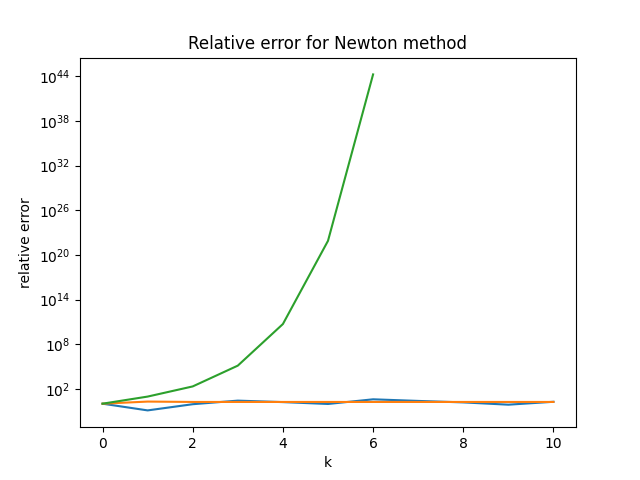
\includegraphics[width=0.8\linewidth]
            {g_relative_error.png}
        \caption{Wartość błędu względnego w zależności od
            numeru iteracji.}
    \end{figure}
    \begin{figure}[H]
        \centering
        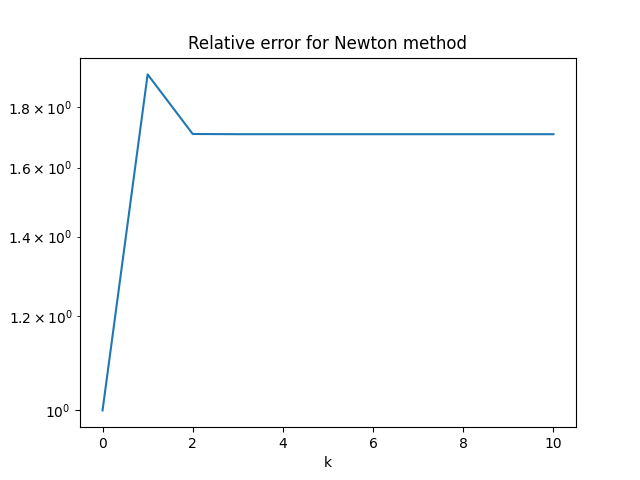
\includegraphics[width=0.8\linewidth]
            {g_convergent.png}
        \caption{Wartość błędu względnego dla metody
            zbieżnej.}
    \end{figure}

    \subsection{Zadanie 3.}
    \begin{table}[H]
        \centering
        \renewcommand{\arraystretch}{1.5}
        \begin{tabular}{|c|c|c|}
            \hline
            Funkcja & Dokładność 24-bitowa & Dokładność
                53-bitowa \\
            \hline
            $f_1$ & $k=3$ & $k=4$ \\
            \hline
            $f_2$ & $k=3$ & $k=4$ \\
            \hline
            $f_3$ & $k=2$ & $k=3$ \\
            \hline
        \end{tabular}
        \caption{Liczba iteracji potrzebna do uzyskania
            wymaganej dokładności dla każdej funkcji.}
    \end{table}

    \subsection{Zadanie 4.}
    Dla początkowego oszacowania $x_0=1$ oraz wykonując
    $k=4$ iteracji udało się uzyskać błąd względny rozwiązania
    $\epsilon \approx 1.87 \cdot 10^{-10}$. Dla $k=5$
    iteracji błąd względny osiągał już wartość 0, czyli
    błąd numeryczny przekraczał wartość błędu metody.

    \section{Wnioski}
    Metoda Newtona jest bardzo skutecznym narzędziem do
    znajdowania miejsc zerowych funkcji. Cechuje ją duża
    szybkość działania, ponieważ metoda posiada kwadratowy
    rząd zbieżności. Należy jednak uważać przy wyborze
    początkowego oszacowania $x_0$, ponieważ w pobliżu
    ekstremów lokalnych funkcji, metoda może się zachowywać
    w sposób nieprzewidywalny i zwracać błędne wyniki.
    W niektórych przypadkach warto rozważyć użycie innej,
    wolniejszej metody, ale bardziej skutecznej.

    \section{Bibliografia}
    \url{https://pl.wikipedia.org/wiki/Metoda_Newtona} \\
    \url{https://en.wikipedia.org/wiki/Rate_of_convergence} \\
    \url{https://pl.wikipedia.org/wiki/
        Liczba_zmiennoprzecinkowa}

\end{document}
